\chapter{Differential- und Integralrechnung für Funktion von mehreren Variablen}
\section{Funktion von mehreren Variablen}
\subsection{Definition}
\begin{definition}
Unter einer Funktion von zwei unabhängigen Variablen versteht man eine Vorschrift, die jedem geordneten Zahlenpaar $(x;y)$ aus einer Menge $D$ genau ein Element $z$ aus einer Menge $W$ zuordnet, Symbolische Schreibweise: $$z=f(x;y)$$
Analog gelangt man zu Funktionen von mehr als zwei unabhängigen Variablen:
$$u=f(x;y;z)$$

\subsection{Darstellungsformen}
Es gibt vier verschiedene Darstellungsformen:
\begin{enumerate}
	\item \textit{Explizit} dargestellt:
	$$z = 2x + y + 1 \text{ oder } z = 2 \cdot sin(x-y)$$
	\item \textit{Implizit} dargestellt:
	$$ x^2 + y^2+z -1 = 0$$
	\item Dargestellt in einer \textit{Funktionstabelle}.
	\item Graphische Darstellung (als Fläche, Höhenlinien, Schnittkurven..).
\end{enumerate}
Die dritte und vierte Form eigenen sich nur für Funktionen mit maximal drei Variablen.
\end{definition}

\subsubsection{Höhenliniendiagramm}
\begin{definition}
Die \textit{Höhenlinien} einer Funktion $z=f(x;y)$ genügen der impliziten Kurvengleichung
$$f(x;y) = const. = c$$
$c$: Wert der Höhenkoordinate $z$ (Kurvenparameter)
\end{definition}
Die \textit{Höhenlinien} sind die Projektionen der \textit{Linien gleicher Höhe} in die $x, y$-Koordinatenebene.

\subsection{Definitions- und Wertebereich}
Der Definitionsbereich $D$ einer Funktion $z = f(x,y)$ kann als eine flächenhafte Punktmenge in der $x, y$-Ebene aufgefasst werden.
\begin{bsp}
$$z = \sqrt{25-x^2-y^2}$$
Definitionsbereich: $ 25-x^2-y^2 \geq 0$, d. h. $x^2 + y^2 \leq 25$.\\
Wertebereich: $ 0 \leq z \leq 5$ (wegen $0\leq 25 -x^2-y^2 \leq 25$).
\end{bsp}

\section{Grenzwert und Stetigkeit einer Funktion}
\subsection{Grenzwert}
\begin{definition}
Eine Funktion zweier Variablen hat an der Stelle $(x_,y_0)$ den Grenzwert $g$, wenn sich die Funktionswerte $f(x,y)$ beim Grenzübergang $(x,y) \rightarrow (x_0,y_0)$ unabhängig vom eingeschlagenen Weg dem Wert $g$ beliebig nähern. Symbolische Schreibweise:
$$\lim\limits_{(x,y) \rightarrow (x_0,y_0)} f(x,y) = g$$
\begin{enumerate}
\item Eine Funktion kann auch in einer Definitionslücke $(x_0,y_0)$ einen Grenzwert haben, obwohl sie dort nicht definiert ist.
\item Grenzwert auf einer Bildfläche: Je näher man zur Stelle $(x_0,y_0)$ kommt, desto flacher wird die Ebene auf der man sich bewegt.
\end{enumerate}
\end{definition}

Um den Grenzwert berechnen zu können, muss an versuchen eine Variable loszuwerden.
\begin{bsp}
$x$ und $y$ können auch in Polarkoordinatenform ausgedrückt werden: $x = r \cdot \text{cos} \phi \text{ und } y = r \cdot \text{sin} \phi$. Die Verwendung des trigonometrischen Pythagoras ($\text{sin}^2 \phi + \text{cos}^2 \phi = 1$) kann sich in diesem Fall anbieten:
$$ x^2 + y^2 =  r^2 \cdot \sin^2 \phi + r^2 \cdot \text{cos}^2 \phi =r^2(\text{sin}^2 \phi + \text{cos}^2 \phi) = r^2$$
Die Grenzwertberechnung vereinfacht sich nun auf eine unabhängige Variable ($\lim\limits_{r\rightarrow n} f(x)$).
\end{bsp}

\subsection{Stetigkeit}
\begin{definition}
Eine in $(x_0,y_0)$ und einer gewissen Umgebung von $(x_0,y_0)$ definierten Funktion $z = f(x;y)$ heisst an der Stelle $(x_0,y_0)$ \textit{stetig}, wenn der \textit{Grenzwert} der Funktion an der Stelle \textit{vorhanden} ist und mit dem dortigen Funktionswert \textit{übereinstimmt}.
$$\lim\limits_{(x,y) \rightarrow (x_0,y_0)} f(x,y) = f(x_0,y_0)$$
Anmerkung:
\begin{enumerate}
\item Die Stetigkeit an einer bestimmten Stelle setzt voraus, dass die Funktion dort auf \textit{definiert} ist. Ferner muss der Grenzwert an dieser Stelle existieren und mit dem Funktionswert übereinstimmen.
\item Eine Funktion $z = f(x,y)$ heisst dagegen an der Stelle $(x_0,y_0)$ \textit{unstetig}, wenn  $f(x_0,y_0)$ \textit{nicht} vorhanden ist oder $f(x_0,y_0)$ vom Grenzwert \textit{verschieden} ist oder dieser \textit{nicht} existiert.
\item Eine Funktion, die an \textit{jeder} Stelle ihres Definitionsbereichs stetig ist, wird als stetige Funktion bezeichnet.
\end{enumerate}
\end{definition}

Für Stetigkeit im Nullpunkt $(0, 0)$ muss gelten: $\lim\limits_{(x,y) \rightarrow (0,0)} f(x) = f(0,0) = a$


\section{Partielle Differentiation}
\subsection{Partielle Ableitung 1. Ordnung}
\begin{definition}
Ist $z = f(x,y)$ an \textit{jeder} Stelle $(x,y)$ einer gewissen Bereiches \textit{partiell} differenzierbar, so sind die partiellen Ableitungen 1. Ordnung selbst wieder \textit{Funktionen} von $x$ und $y$. 
$$ z_x = \frac{\partial z}{\partial x} = \frac{\partial z}{\partial u} \cdot \frac{\partial u}{\partial x}$$
$$ z_x = \frac{\partial z}{\partial x} = \frac{\partial z}{\partial x} \cdot \frac{\partial v}{\partial u} \cdot \frac{\partial u}{\partial x}$$

Übliche Symbole für partielle Ableitungen sind:
$$f_x(x, y) \text{ , } z_x(x, y) \text{ , } \frac{\partial f}{\partial x} (x, y) \text{, } \frac{\partial z}{\partial y} (x, y)$$
\end{definition}

\begin{bsp}
$z = \sqrt{2xy -y^2} \text{ ;  } u = 2xy - y^2 \Rightarrow z = \sqrt{u}$
\begin{align*}
	z_x &= \frac{\partial z}{\partial x} = \frac{\partial z}{\partial u} \cdot \frac{\partial u}{\partial x} = \frac{1}{2 \sqrt{u}} \cdot 2y = \frac{y}{\sqrt{u}} = \frac{y}{\sqrt{2xy-y^2}} \\
	z_y &= \frac{\partial z}{\partial y} = \frac{\partial z}{\partial u} \cdot \frac{\partial u}{\partial y} = \frac{1}{2 \sqrt{u}} \cdot (2x-2y) = \frac{x-y}{\sqrt{u}} = \frac{x-y}{\sqrt{2xy-y^2}}
\end{align*}
\end{bsp}

\begin{bsp}
Von  $ z = -4x^3y^2 + 3xy^4 - 3x +2y +5$ die partielle Ableitung 1. Ordnung bestimmen und die Werte an der Stelle $x=1$, $y=2$ berechnen:
\begin{itemize}
		\item $f_x= -12x^2y^2+3y^4-3$
		\item $f_y = -8x^3y + 12xy3 +2$
		\item $f_x(1;2) = -3$, $f_y(1,2) = 82$, Höhenkoordinate: $z = f(1;2) = 38$
		\item Die im Flächenpunkt $P = (1, 2, 38)$ errichteten Tangenten besitzen den folgenden Anstieg, bzw Steigungswinkel:
		\begin{itemize}
			\item Tangente in $x$-Richtung: $m_x = \text{tan} \alpha = -3 \Rightarrow \alpha = 180^\circ + \text{arctan}(-3) = 180^\circ - 71.6^\circ = 108.4^\circ$
			\item Tangente in $y$-Richtung: $m_y =  \text{tan} \beta = 82 \Rightarrow \beta = \text{arctan} 82 = 89.3^\circ$
		\end{itemize}
\end{itemize}
\end{bsp}

\subsection{Partielle Ableitungen höherer Ordnung}
\begin{definition}
Es wird genau gleich vorgegangen wie bei der Ableitung erster Ordnung. Die einzelnen Differentiationsschritte sind in der Reihenfolge, in der die als Indizes angehängten Differentiationsvariablen im Ableitungssymbol auftreten, auszuführen. 

$f_{xy}$: Hier wird zunächst nach der Variablen $x$ und anschliessend nach der Variablen $y$ differenziert.

Partielle Ableitungen höherer Ordnung lassen sich auch in der Form partielle Differentialquotienten darstellen:
$$
f_{xx} = \frac{\partial}{\partial x} \left( \frac{\partial f}{\partial x} \right) = \frac{\partial^2 f}{\partial x^2} 
\text{ , } 
f_{xy} = \frac{\partial}{\partial y} \left( \frac{\partial f}{\partial x} \right) = \frac{\partial^2 f}{\partial x \partial y} 
$$
Beispiel 3. Ordnung:
$$ f_{xyx} = \frac{\partial^3 f}{\partial x \partial y \partial x} $$
\end{definition}

\subsubsection{Satz von Schwarz}
\begin{definition}
Bei einer gemischten partiellen Ableitung $k$-ter Ordnung darf die Reihenfolge der einzelnen Differentiationsschritte vertauscht werden, wenn die partiellen Ableitungen $k$-ter Ordnung stetige Funktionen sind.
$$ f_{xy} = f_{yx} \text{, }  f_{xxy} = f_{yxx} \text{, usw...}$$
\end{definition}

\subsection{Das totale/vollständige Differential einer Funktion}
\begin{definition}
Die Gleichung der Tangentialebene an die Fläche $z = f(x, y)$ im Flächenpunkt $P=(x_0, y_0, z_0)$ mit $z_0 = f(x_0, y_0)$ lautet in symmetrischer Schreibweise:
$$\Delta z = t(x, y) = f_x(x_0, y_0) \cdot (x-x_0) + f_y(x_0, y_0) \cdot (y - y_0) + f(x_0, y_0)$$
Um $z$ zu erhalten, müssen nur $x_0$ und $y_0$ in die Ursprungsfunktion $f(x,y)$ eingesetzt werden!

\end{definition}

\subsubsection{Vollständiges Differential}
\begin{definition}
Bei einer Funktion  $z=f(x,y)$ von zwei unabhängigen Variablen beschreibt das totale Differential:
$$ dz = f_x(x_0, y_0) dx + f_y(x_0, y_0) dy$$
die Änderung der Höhenkoordinate bzw. des Funktionswerts $z$ auf der im Berührungspunkt $P = (x_0, y_0, z_0)$ errichteten Tantentialebene. Dabei sind die "Differentiale"  $ dx, dy, dz$ die Koordinaten eines beliebigen Punktes auf der Tangentialebene, bezogen auf den Punkt $P$.

Hier kommt noch das Bild von Slide 14

Bei $n$ unabhängigen Variablen versteht man den linearen Differentialausdruck
$$dy = f_{x_1} dx_1 + f_{x_2} dx_2 + ... + f_{x_n} dx_n = \frac{\partial f}{\partial x_1} dx_1 + \frac{\partial f}{\partial x_2} dx_2 + ... + \frac{\partial f}{\partial x_n} dx_n$$

Bemerkung: $f(x+dx, y+dy) - f(x,y) = \Delta z \approx dz$
\end{definition}

\subsubsection{Implizite Differentiation}
\begin{definition}
Der Anstieg einer in der impliziten Form $F(x, y) = 0$ dargestellten Funktionskurve im Kurvenpunkt $P=(x,y)$ lässt sich wie folgt bestimmen:
$$y'(P) = - \frac{F_x(x,y)}{F_y(x,y)}$$
\end{definition}

\subsubsection{Linearisierung einer Funktion}
\begin{definition}
In der Umgebung des Kurvenpunktes $P=(x_0,y_0)$ kann die nichtlineare Funktion $y=f(x)$ nährungsweise durch die lineare Funktion (Kurventangente)
$$y -y_0 = f'(x_0) \cdot (x - x_0) \text{ oder } \Delta y = f'(x_0)$$
ersetzt werden. 

Analog können wir eine nichtlineare Funktion $z=f(x,y)$ in der Nähe des Punktes $P=(x_0, y_0, z_0)$ durch die Tangentialebene annähern:
$$z=f(x,y) = f_x(x_0, y_0) \cdot (x-x_0) + f_y(x_0, y_0) \cdot (y-y_0) + z_0$$
auch 
$$ V= f_x(x_0, y_0, z_0) \cdot \Delta x + f_y(x_0, y_0, z_0) \cdot \Delta y + f_z(x_0, y_0, z_0) \cdot \Delta z$$
\end{definition}

\subsubsection{Relative Extremwerte}
\begin{definition}
Wie bei Analysis 1 gibt es zwei Bedingungen für Extremwerte:
\begin{itemize}
	\item \textbf{Notwendige} Bedingung: $f_x(x_0, y_0) = 0 \wedge f_y(x_0, y_0) = 0$
	\item \textbf{Hinreichende} Bedingung: $f_{xx}(x_0, y_0) \cdot f_{yy}(x_0, y_0)  - (f_{xy}(x_0, y_0))^2 > 0 = \Delta$
	\item  Das Vorzeichen von \textbf{$f_{xx}(x_0, y_0)$} entscheidet über die Art des Extremwertes:
	\begin{itemize}
		\item $f_{xx}(x_0, y_0) < 0 \Rightarrow $ relatives \textbf{Maximum}
		\item $f_{xx}(x_0, y_0) > 0 \Rightarrow $ relatives \textbf{Minimum}
		\item falls $\Delta < 0 \Rightarrow$ Sattelpunkt
		\item falls $\Delta = 0 \Rightarrow$ keine Aussage möglich
		\end{itemize}
\end{itemize}
\end{definition}

\subsection{Doppelintegrale}
Wenn wir ein Doppelintegral berechnen wollen, müssen wir wissen, wie der Integrationsbereich $A$ aussieht und führen dann zwei Integrationsschritte durch.
\begin{itemize}
	\item \textbf{1. Fall:} $x$ liegt zwischen konstanten Grenzen, $y$ zwischen zwei Funktionen
	$$ \iint_{(A)} f(x,y) dA$$ 
	\item \textbf{2. Fall:} $x$ liegt zwischen zwei Funktionen, $y$ zwischen konstanten Grenzen.
\end{itemize}

\subsubsection{Allgemein}
\begin{enumerate}
	\item Fall: Wir müssen zuerst nach $y$ integrieren (inneres Integral) und danach das äussere Integral nach $x$ integrieren.
	\item Fall:Wir müssen zuerst nach $x$ integrieren (inneres Integral) und danach das äussere Integral nach $y$ integrieren.
\end{enumerate}

\subsubsection{Doppelintegrale in Polarkoordinaten}
Je nach Problemstellung vereinfacht sich die Berechnung eines Doppelintegrals erheblich, wenn man an Stelle der kartesischen Koordinaten die Polarkoordiaten verwendet:
\begin{itemize}
\item $x = r \cdot cos\phi$
\item $y = r \cdot sin\phi$
\item $r^2 = x^2 + y^2$
\item $r \geq 0$ und $0 \leq \phi < 2\pi$
\end{itemize}
Integrationsbereiche bei denen diese Form angewendet werden kann werden von zwei Strahlen $\phi_1$ und $\phi_2$, sowie einer inneren Kurve $r_i(\phi)$ und einer äusseren Kurve $r_a(\phi)$ begrenzt. Für das infinitesimale Flächenelement gilt: $dA = (rd\phi) \cdot dr = rd\phi dr$. Das Doppelintegral besitzt die folgende Form:
$$\iint\limits_{(A)} f(x, y) da = \int\limits_{\phi = \phi_1}^{\phi2} \int\limits_{r = r_i(\phi)}^{r_a(\phi)} f(r\cdot cos\phi, r \cdot sin \phi) \cdot r \cdot dr d\phi$$
\begin{figure}[H]
\centering
	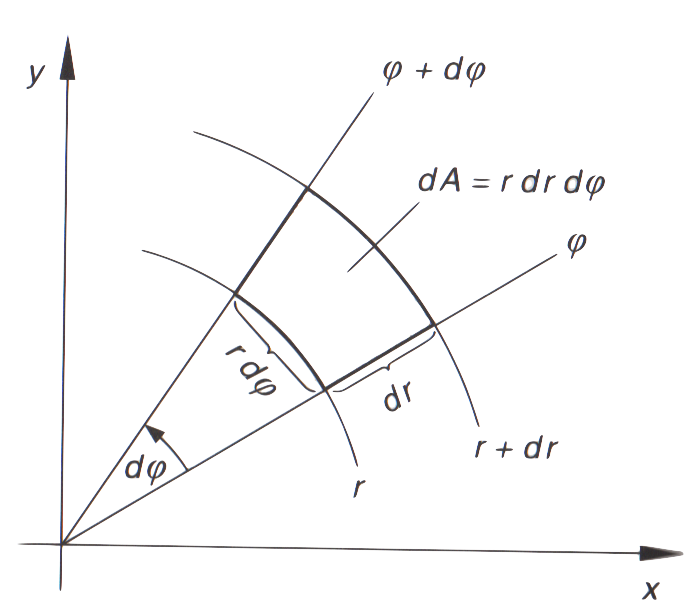
\includegraphics[width=5cm]{Bilder/dipolar_1}
	\caption{Flächenelemen $dA$ in Polarkoordinaten}
	\label{dipolar1}
\end{figure} 

